\section{Math}

  Type \textbackslash( to start inline math and Texpile recognizes it immediately: \(E = mc^2\).
Display math gets its own line:
\[
        \int_0^\infty e^{-x^2}\,dx = \frac{\sqrt{\pi}}{2}
  \]

\section{Figures and references}

Drag an image file from your file manager straight into the editor to insert it directly; this one
      was added that way. Copy an image and paste it (Ctrl+V) works too.

\begin{figure}[h]
		\centering
	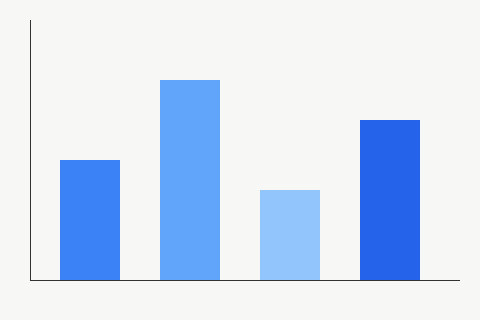
\includegraphics[width=0.6\textwidth]{images/sample.png}
			\caption{Image paths resolve relative to this folder, the same as \texttt{\textbackslash input}.}
	\label{fig:sample}
	\end{figure}

  In Source mode, typing \texttt{\textbackslash ref\{} or \texttt{\textbackslash cite\{}
autocompletes from this project's own labels and \texttt{references.bib}: see
Figure~\ref{fig:sample}, or \citep{doe2024} and \citet{smith2023} for both citation styles.
